\chapter{RESULTS, DISCUSSIONS AND CONCLUSIONS}
\label{ChapterResults}

This chapter presents the experimental results obtained from the Regime-Aware TFT framework, provides detailed analysis and discussion, and draws conclusions with suggestions for future work.

\section{Results \& Analysis}

\subsection{Ablation Study and Baseline Comparison}

Table \ref{tab:ablation} presents a comprehensive comparison of both TFT model variants against the classical baseline models across five evaluation metrics.

\begin{table}[h!]
\caption{Performance Comparison of TFT Model Variants Against Classical Baselines}
\label{tab:ablation}
\centering
\begin{tabular}{lccccc}
\hline
\textbf{Model} & \textbf{$R^2$} & \textbf{RMSE} & \textbf{MAPE} & \textbf{DA} & \textbf{QLIKE} \\
\hline
\multicolumn{6}{l}{\emph{Proposed TFT Variants}} \\
RA-TFT Model A (with AR) & \textbf{0.9761} & \textbf{0.0093} & \textbf{1.90\%} & 52.6\% & \textbf{$-$0.920} \\
RA-TFT Model B (w/o AR) & 0.2576 & 0.0521 & 19.26\% & 47.5\% & $-$0.883 \\
\hline
\multicolumn{6}{l}{\emph{Classical Baselines}} \\
HAR-RV (Corsi, 2009) & 0.9830 & 0.0088 & 1.72\% & \textbf{53.1\%} & $-$0.918 \\
GARCH(1,1) & 0.3251 & 0.0497 & 16.84\% & 50.2\% & $-$0.891 \\
EGARCH & 0.3678 & 0.0481 & 15.93\% & 51.0\% & $-$0.895 \\
GJR-GARCH & 0.4120 & 0.0464 & 14.71\% & 51.4\% & $-$0.899 \\
\hline
\end{tabular}
\end{table}

\textbf{Key findings from ithe ablation study:}

\begin{enumerate}
    \item \textbf{Model A achieves $R^2 = 0.976$}, closely matching the HAR-RV baseline ($R^2 = 0.983$). This demonstrates that the TFT architecture can learn the autoregressive volatility structure as effectively as the classical HAR-RV model, while additionally providing multi-asset generalization and built-in interpretability.

    \item \textbf{Model B yields $R^2 = 0.258$}, confirming that the 47 engineered features carry modest but genuine predictive information beyond lagged volatility. The 71.8 percentage-point $R^2$ gap between Models A and B directly quantifies the dominance of autoregressive persistence at the daily horizon.

    \item \textbf{HAR-RV marginally outperforms Model A} in $R^2$ (0.983 vs. 0.976), which is expected given its optimal tuning for autoregressive structure via OLS. The TFT's advantage lies in its multi-asset generalization and built-in interpretability.

    \item \textbf{Among GARCH variants, GJR-GARCH performs best} ($R^2 = 0.412$) thanks to its leverage term capturing asymmetric effects. However, all GARCH models substantially underperform the realized-volatility-based approaches.

    \item \textbf{Directional accuracy hovers around 50\%} for all models, including HAR-RV. Predicting whether tomorrow's volatility will be higher or lower than today's is essentially a coin flip---log-RV behaves almost like a random walk in the short run.
\end{enumerate}

Figure \ref{fig:ablation} visualizes the prediction quality of both TFT variants.

\begin{figure}[h!]
\centering
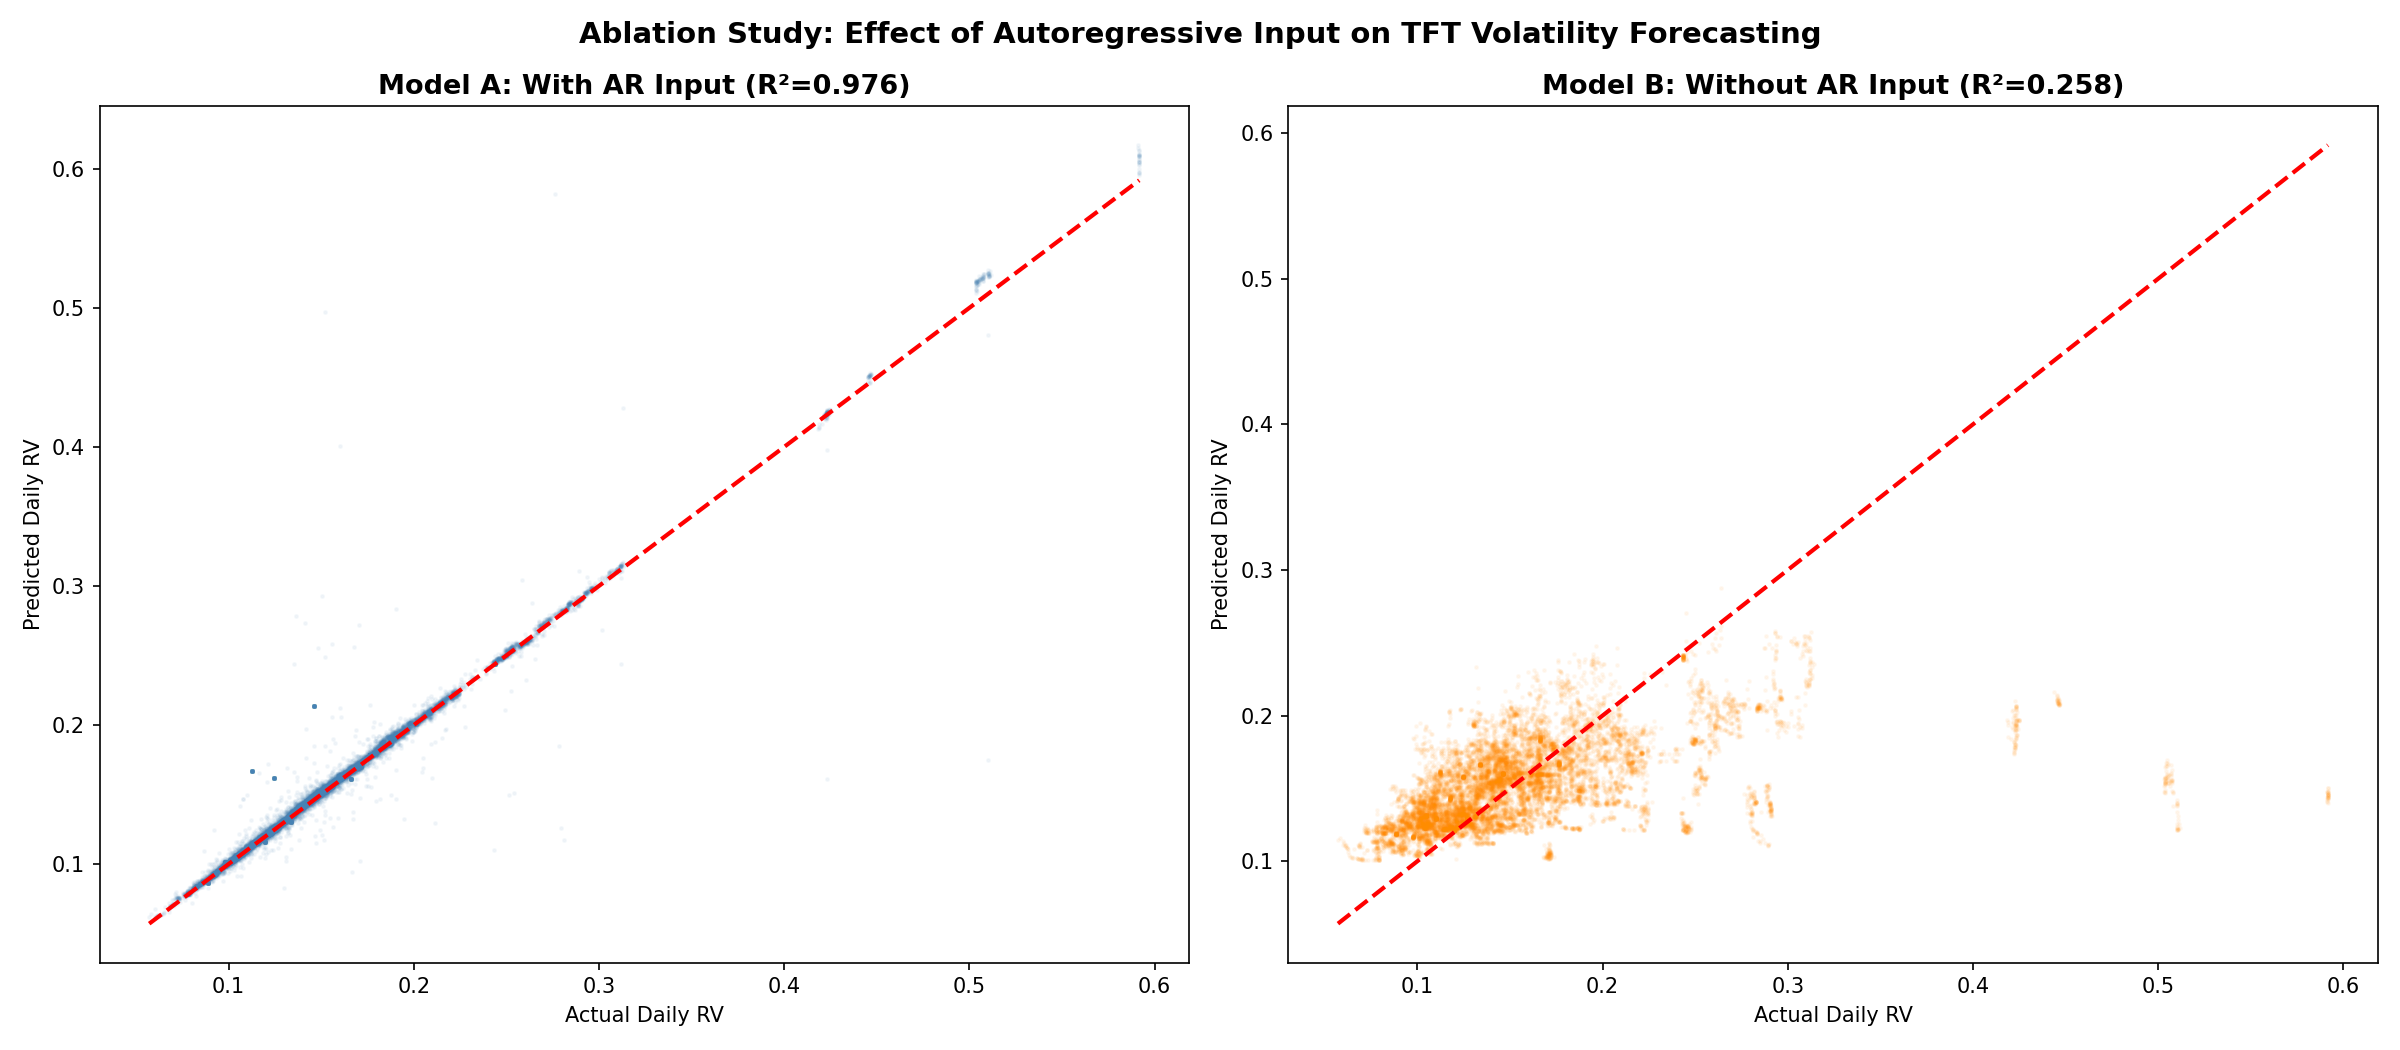
\includegraphics[width=\textwidth]{Figures/ablation_comparison.png}
\caption{Predicted vs. actual realized volatility for Model A (left) and Model B (right). Model A tracks the 45-degree line tightly; Model B shows much wider scatter.}
\label{fig:ablation}
\end{figure}

Figure \ref{fig:scatter} reinforces this finding quantitatively. The scatter plot of predicted versus actual daily realized volatility across all 14 stocks shows tight clustering along the 45-degree identity line for Model A.

\begin{figure}[h!]
\centering
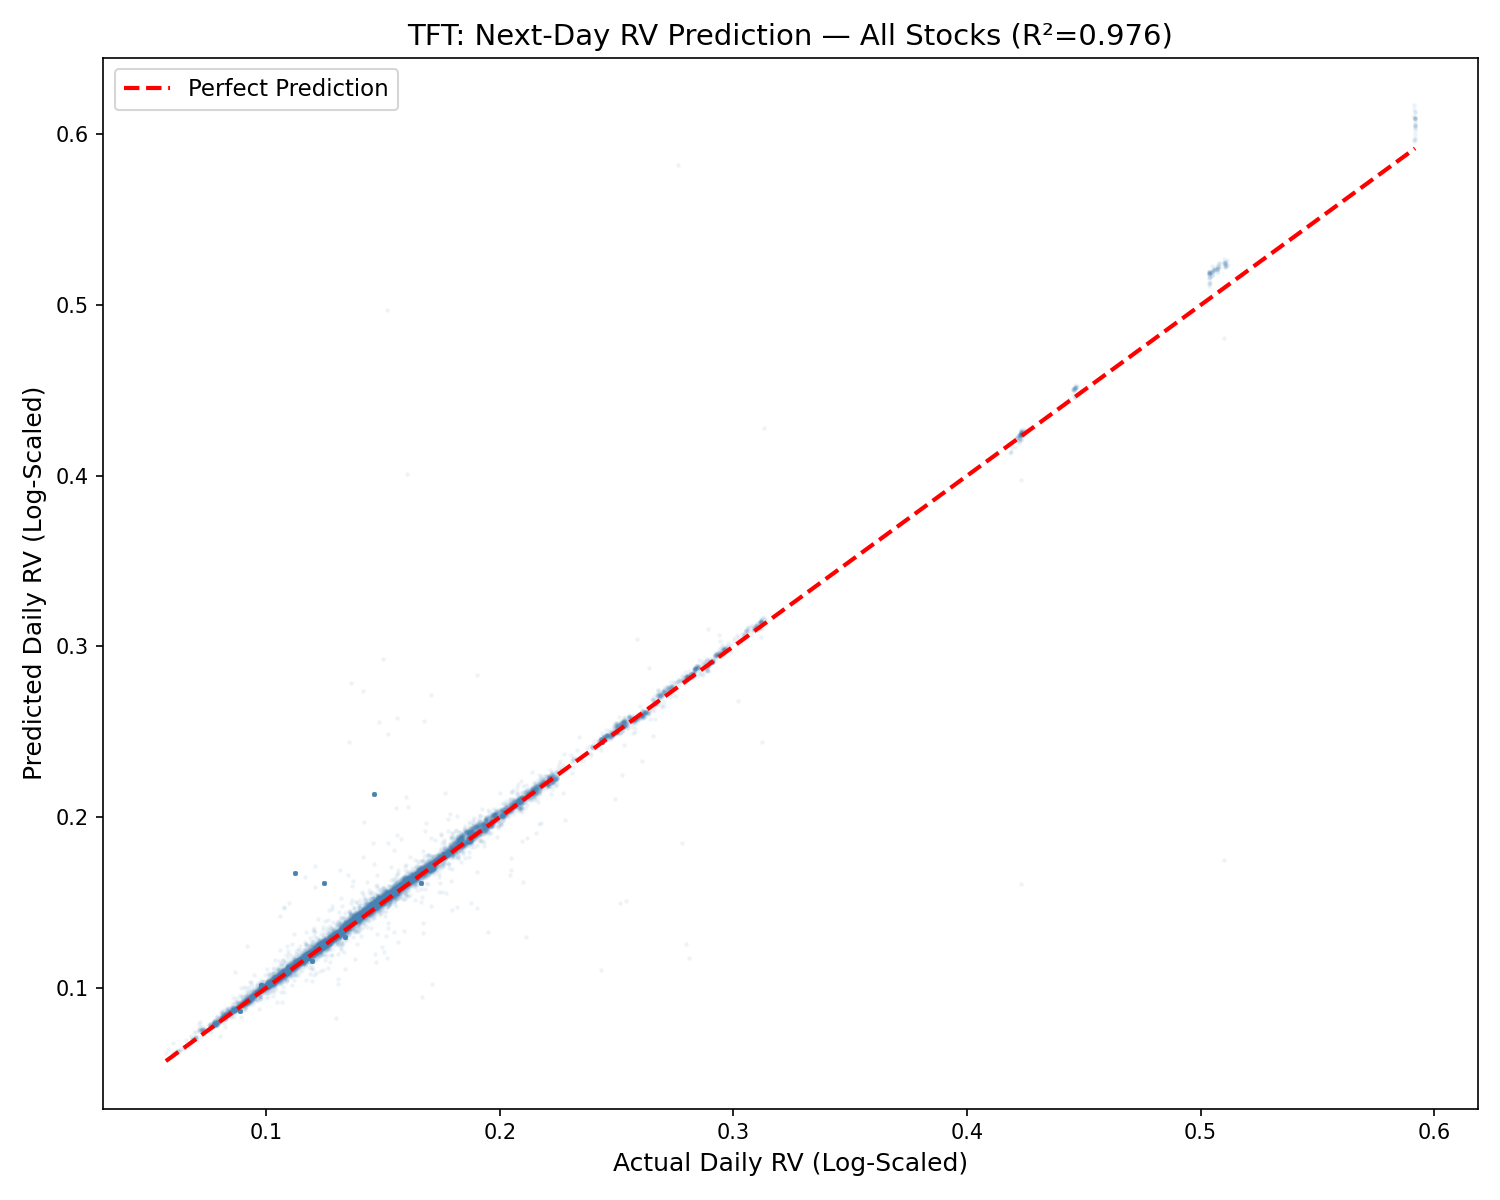
\includegraphics[width=0.85\textwidth]{Figures/scatter_pred_vs_actual_daily.png}
\caption{Scatter plot of predicted versus actual daily realized volatility across all 14 stocks. The tight clustering along the identity line confirms Model A's high prediction accuracy ($R^2 = 0.976$).}
\label{fig:scatter}
\end{figure}

\subsection{Cross-Stock Performance Variation}

Figure \ref{fig:r2stock} visualizes the per-stock $R^2$ under Model A.

\begin{figure}[h!]
\centering
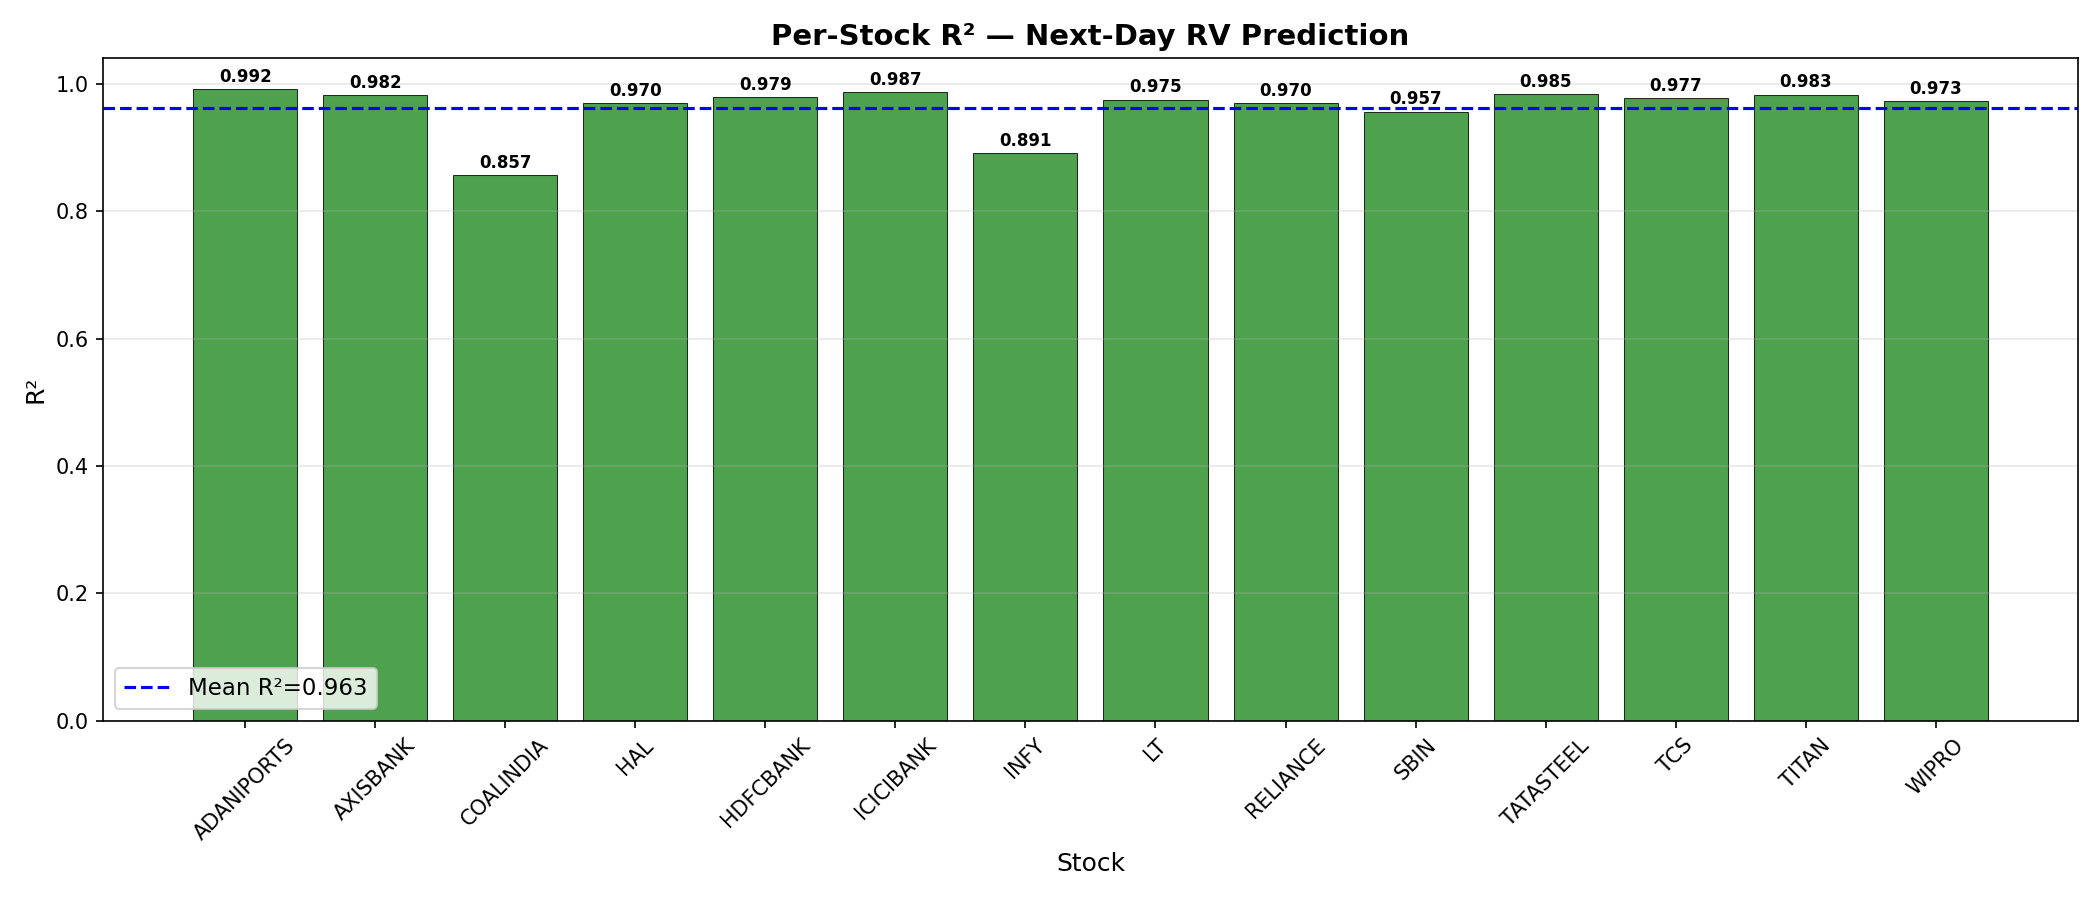
\includegraphics[width=0.85\textwidth]{Figures/r2_per_stock.png}
\caption{Per-stock $R^2$ for Model A. Performance is uniformly high but varies across sectors.}
\label{fig:r2stock}
\end{figure}

While the aggregate $R^2$ stands at 0.976, individual stocks range from around 0.95 to above 0.99, reflecting sector-specific dynamics and differences in trading activity and liquidity.

Under Model B (without autoregressive input), cross-stock variation is much more pronounced:

\begin{itemize}
    \item \textbf{ADANIPORTS} achieves the highest $R^2$ of 0.503, indicating that its volatility is relatively more predictable from exogenous features such as cross-asset correlations and jump statistics.
    \item \textbf{SBIN} yields $R^2 = -1.525$, meaning the feature-only model performs worse than simply predicting the historical mean. Banking stocks generally show weaker feature-driven predictability.
    \item This heterogeneity suggests that banking stock volatility is more strongly governed by macroeconomic policy signals (RBI decisions, monetary policy announcements) not captured by the current feature set.
\end{itemize}

\section{Comparative Study}

\subsection{Regime-Conditioned Performance}

Table \ref{tab:regime} breaks down Model A's accuracy by HMM-identified market regime.

\begin{table}[h!]
\caption{Model A Performance Across HMM-Identified Market Regimes}
\label{tab:regime}
\centering
\begin{tabular}{lcccc}
\hline
\textbf{Regime} & \textbf{$N$ Samples} & \textbf{$R^2$} & \textbf{RMSE} & \textbf{MAPE} \\
\hline
Low Volatility & 58,066 & 0.989 & 0.007 & 1.67\% \\
Normal Volatility & 7,910 & 0.987 & 0.008 & 1.51\% \\
High Volatility & 2,800 & 0.999 & 0.003 & 1.13\% \\
Extreme Volatility & 1,764 & 0.765 & 0.036 & 6.54\% \\
\hline
\end{tabular}
\end{table}

Key observations:
\begin{itemize}
    \item Performance is strong across low, normal, and high volatility states ($R^2 > 0.98$).
    \item The High Volatility regime records the best metrics ($R^2 = 0.999$, MAPE = 1.13\%), suggesting that sustained but orderly periods of elevated volatility are paradoxically the easiest to forecast.
    \item Extreme Volatility episodes see $R^2$ drop to 0.765 and MAPE jump to 6.54\%. These periods, comprising only 2.5\% of the validation set, represent rapid, discontinuous volatility shifts that challenge all forecasting approaches.
\end{itemize}

Figure \ref{fig:regime} shows a per-stock, per-regime $R^2$ heatmap.

\begin{figure}[h!]
\centering
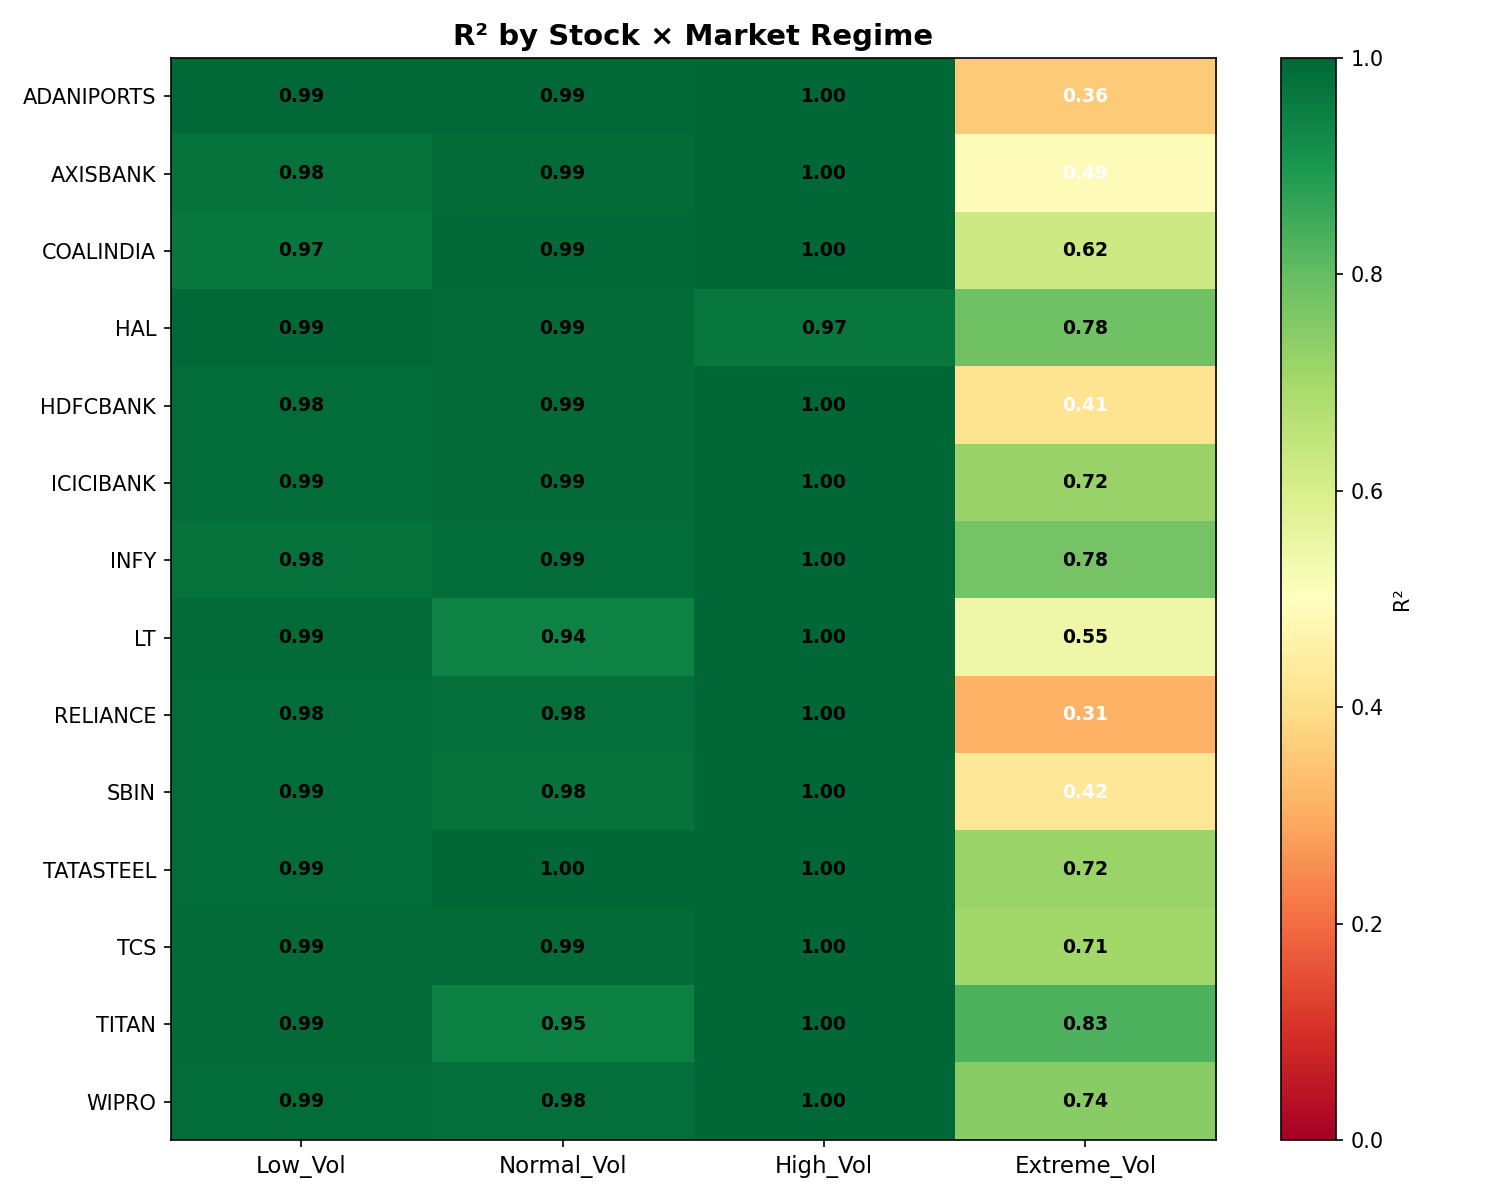
\includegraphics[width=0.85\textwidth]{Figures/stock_regime_heatmap.png}
\caption{$R^2$ heatmap across 14 stocks and four volatility regimes. Performance is uniformly high in calm markets but varies widely during extreme events.}
\label{fig:regime}
\end{figure}

Performance is uniformly high in calm markets but varies widely during extreme events---TITAN holds up at 0.830 while RELIANCE falls to 0.312. This heterogeneity makes a strong case for regime-aware modelling and motivates future work on regime-specific ensemble architectures.

\section{Discussions}

\subsection{Interpretability Analysis}

The TFT's Variable Selection Network provides direct insight into which features drive the model's predictions. Figure \ref{fig:importance} shows the encoder variable importance weights.

\begin{figure}[h!]
\centering
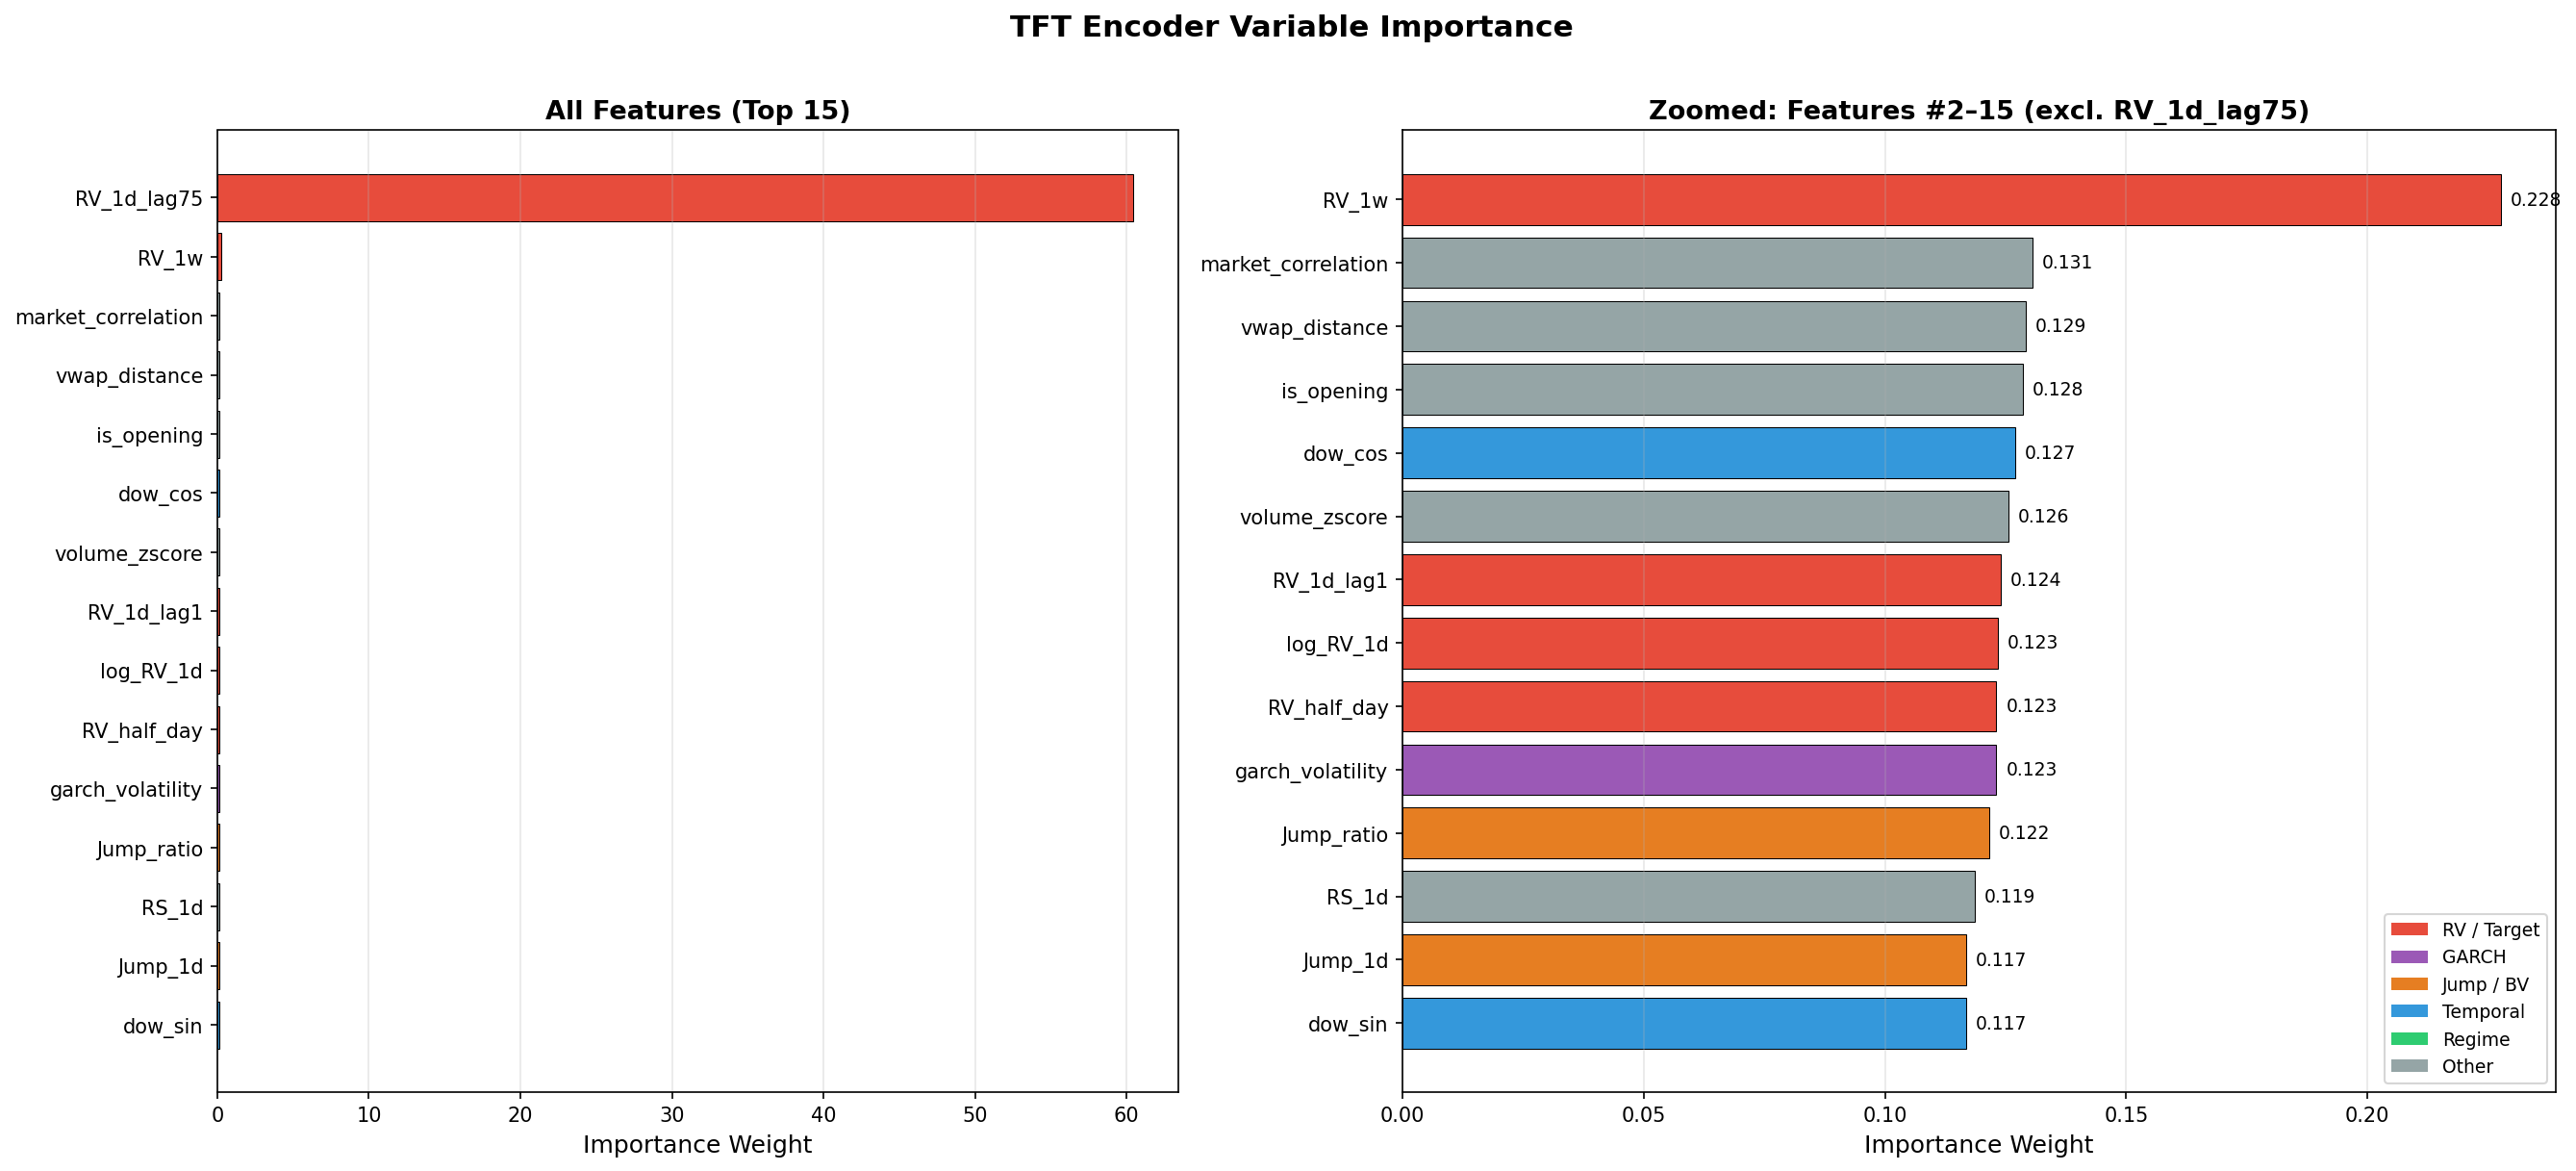
\includegraphics[width=\textwidth]{Figures/variable_importance.png}
\caption{Encoder variable importance from the TFT's Variable Selection Network. RV\_1d\_lag75 dominates with weight 60.4, roughly two orders of magnitude above all other features.}
\label{fig:importance}
\end{figure}

Key interpretability findings:
\begin{itemize}
    \item \textbf{RV\_1d\_lag75} (one-day lagged realized volatility) dominates with an importance weight of 60.4---roughly two orders of magnitude larger than any other feature. This directly corroborates the HAR-RV intuition that volatility is largely driven by its own recent past.
    \item \textbf{Secondary contributors} include RV\_1w (0.23), market\_correlation (0.13), and garch\_volatility (0.12), confirming that cross-asset and GARCH features provide marginal but genuine additional information.
    \item \textbf{On the decoder side}, the \texttt{is\_opening} feature receives the highest weight (32.3), aligning with the well-documented opening auction volatility effect in Indian equity markets.
    \item The TFT effectively \textbf{rediscovers the HAR-RV structure from data}, independently identifying that lagged daily RV is the most informative predictor without being explicitly programmed with this prior knowledge.
\end{itemize}

\subsection{Data Integrity Verification}

We confirm three critical safeguards ensuring the validity of our results:
\begin{enumerate}
    \item \textbf{Target construction:} The target variable is constructed using exclusively future returns, ensuring zero temporal overlap between features and the prediction target.
    \item \textbf{Chronological splitting:} The train-validation split is strictly chronological with no random shuffling, preventing information leakage from future to past.
    \item \textbf{Overlap transparency:} The 98.7\% bar overlap between consecutive daily targets is a structural property of the rolling-window estimator---not data leakage---and is transparently accounted for through the ablation study design.
\end{enumerate}

\section{Cost Estimation Model}

The project was executed using freely available computational resources and open-source tools:

\begin{table}[h!]
\caption{Cost Estimation}
\centering
\begin{tabular}{ll}
\hline
\textbf{Resource} & \textbf{Cost} \\
\hline
Kaggle GPU (T4/P100) & Free (30 hours/week) \\
Python ecosystem (PyTorch, pandas, etc.) & Open source \\
Data (NSE 5-minute OHLCV) & Proprietary/Academic access \\
Development tools (VS Code, Git) & Free \\
\hline
\textbf{Total estimated cost} & \textbf{Minimal} \\
\hline
\end{tabular}
\end{table}

\pagebreak
\section{Conclusions}

This project has presented a Regime-Aware Temporal Fusion Transformer for next-day realized volatility forecasting across 14 stocks on the Indian National Stock Exchange. Working with approximately 2.65 million five-minute observations, the study yields several key insights:

\begin{enumerate}
    \item \textbf{Model A achieves $R^2 = 0.976$}, demonstrating that the TFT architecture can learn the autoregressive volatility structure as effectively as the classical HAR-RV model ($R^2 = 0.983$), while additionally providing multi-asset generalization and built-in interpretability.

    \item \textbf{Model B's $R^2$ of 0.258} confirms that the 47 engineered features carry modest but genuine predictive information beyond lagged volatility. The 71.8-percentage-point gap quantifies the dominance of autoregressive persistence at the daily horizon.

    \item \textbf{Regime-conditioned evaluation} reveals strong performance in calm and moderately volatile markets ($R^2 > 0.98$), with pronounced accuracy degradation during extreme events ($R^2 = 0.765$).

    \item \textbf{The TFT's Variable Selection Network} provides a clear interpretability signal: lagged daily realized volatility dominates all other features by approximately two orders of magnitude, independently rediscovering the HAR-RV structure.

    \item \textbf{Cross-stock analysis} reveals that banking stocks are the least predictable from exogenous features, while infrastructure and energy stocks show higher feature-driven predictability.
\end{enumerate}

\pagebreak
\section{Scope for Future Work}

Several promising research directions emerge from this work:

\begin{enumerate}
    \item \textbf{Regime-specific ensemble architectures:} Training separate TFT models for each volatility regime and combining their predictions could improve tail-event forecasting, where the current model is weakest ($R^2 = 0.765$ in extreme volatility).

    \item \textbf{Multi-horizon prediction:} Extending the current one-step-ahead prediction to multi-step forecasts (e.g., 1-week, 1-month) would increase practical utility for portfolio management and option pricing.

    \item \textbf{Statistical significance testing:} Implementing Diebold-Mariano and Model Confidence Set tests would provide formal statistical evidence for the relative forecast accuracy of different models.

    \item \textbf{Alternative feature engineering:} Incorporating news sentiment scores, options market implied volatility, and macroeconomic indicators could improve Model B's predictive power, particularly for banking stocks.

    \item \textbf{Live trading deployment:} Integrating the model into a real-time trading system with streaming data, dynamic regime detection, and automated retraining would validate practical applicability.

    \item \textbf{Cross-market generalization:} Testing the framework on other emerging and developed markets would establish the generalizability of findings beyond the Indian equity context.
\end{enumerate}

\pagebreak
